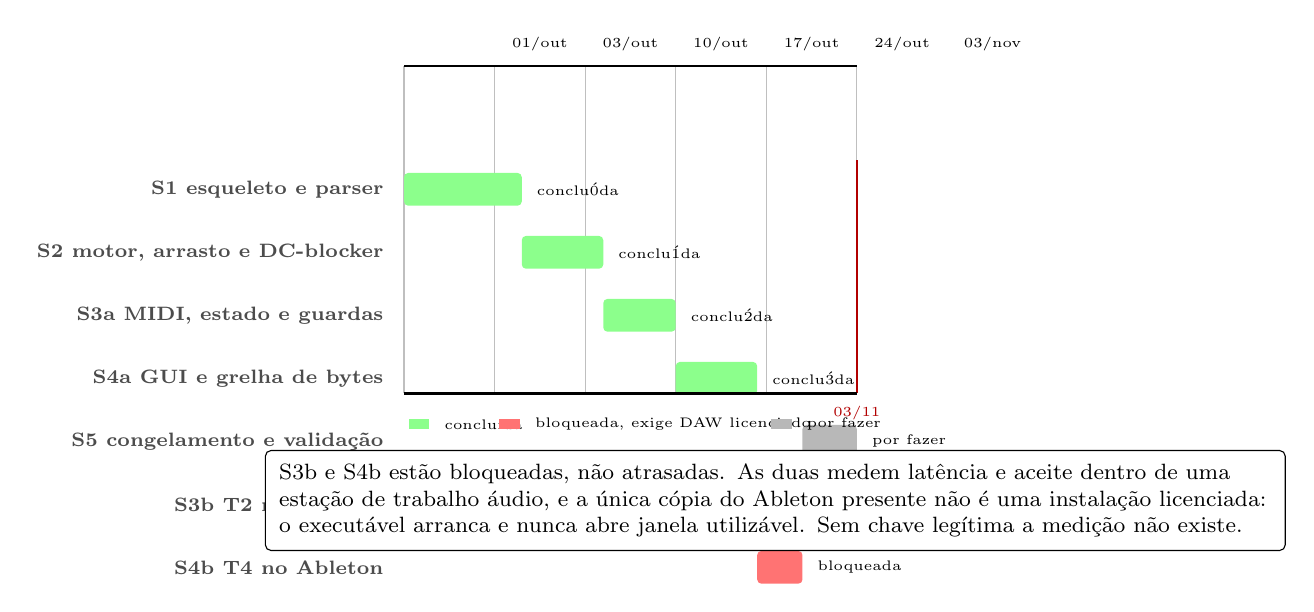
\begin{tikzpicture}[x=1.15cm, y=0.80cm]
  % Grade de datas: de 01/10 a 03/11/2026
  \foreach \x in {0,...,5} {
    \draw[black!25] (\x,0.55) -- (\x,-4.65);
  }
  \foreach \d [count=\xi start=0] in {01/out,03/out,10/out,17/out,24/out,03/nov} {
    \node[font=\tiny] at ({\xi+0.5},0.90) {\d};
  }
  \draw[thick] (0,0.55) -- (5,0.55);

  % Etapas: rotulo / inicio / fim / cor / estado
  \def\etapas{
    {S1 esqueleto e parser}/0/1.3/{green!45}/{concluída},
    {S2 motor, arrasto e DC-blocker}/1.3/2.2/{green!45}/{concluída},
    {S3a MIDI, estado e guardas}/2.2/3.0/{green!45}/{concluída},
    {S4a GUI e grelha de bytes}/3.0/3.9/{green!45}/{concluída},
    {S5 congelamento e validação}/4.4/5.0/{black!28}/{por fazer},
    {S3b T2 no Ableton}/3.0/3.5/{red!55}/{bloqueada},
    {S4b T4 no Ableton}/3.9/4.4/{red!55}/{bloqueada}
  }
  \foreach \t/\a/\b/\cor/\s [count=\i from 0] in \etapas {
    \pgfmathsetmacro{\y}{-\i-1.15}
    \node[font=\scriptsize\bfseries, text=black!70, anchor=east] at (-0.12,{\y-0.26}) {\t};
    \fill[\cor, rounded corners=1.5pt] (\a,\y) rectangle (\b,{\y-0.52});
    \node[font=\tiny, anchor=west] at ({\b+0.06},{\y-0.26}) {\s};
  }

  % Marco de entrega
  \draw[thick, red!70!black] (5,-0.95) -- (5,-4.65);
  \node[font=\tiny, text=red!70!black, anchor=north] at (5,-4.70) {03/11};
  \draw[thick] (0,-4.65) -- (5,-4.65);

  % Legenda de estado
  \fill[green!45] (0.05,-5.05) rectangle (0.28,-5.22);
  \node[font=\tiny, anchor=west] at (0.34,-5.14) {concluída};
  \fill[red!55] (1.05,-5.05) rectangle (1.28,-5.22);
  \node[font=\tiny, anchor=west] at (1.34,-5.14) {bloqueada, exige DAW licenciado};
  \fill[black!28] (4.05,-5.05) rectangle (4.28,-5.22);
  \node[font=\tiny, anchor=west] at (4.34,-5.14) {por fazer};

  % Nota sobre o bloqueio
  \node[draw, fill=white, rounded corners=2pt, align=left, font=\footnotesize, inner sep=5pt, text width=12.6cm] at (4.1,-6.35)
    {S3b e S4b estão bloqueadas, não atrasadas. As duas medem latência e aceite dentro de uma estação de trabalho áudio, e a única cópia do Ableton presente não é uma instalação licenciada: o executável arranca e nunca abre janela utilizável. Sem chave legítima a medição não existe.};
\end{tikzpicture}
